\documentclass[aspectratio=169]{beamer}
\usetheme{metropolis}
\usepackage{geometry}
\usepackage{amsmath}
\usepackage{graphicx}
\graphicspath{ {./figures2/} }
\usepackage{amsfonts}
\usepackage{amssymb}
\usepackage{setspace}
\usepackage{theorem}
\usepackage{natbib}
\usepackage{mathtools}
\usepackage{cite}
\usepackage{natbib}
\usepackage{setspace}
\usepackage[utf8]{inputenc}
\usepackage[english]{babel}
\usepackage{array}
\usepackage{caption}
\usepackage{siunitx}
\usepackage[normalem]{ulem}
\usepackage{multirow}
\usepackage{hhline}
\usepackage{calc}
\usepackage{tabularx}
\usepackage{threeparttable}
\usepackage{wrapfig}
\usepackage{adjustbox}
\usepackage{hyperref}
\usepackage{tikz}
\usepackage[table]{xcolor}

\title{Learning with Misspecified Models:\\  
the case of overconfidence}
\author{Jimena Galindo}

  
\begin{document}

\frame{\titlepage}

\begin{frame}{Overconfidence is Costly}
    \textbf{OVERCONFIDENCE}: Belief that my type is higher than it truly is (``overestimation'' as in Moore and Healy (2008))\\
    \bigskip
    \pause
    It seems to be persistent in various settings. 
    \begin{itemize} 
        \item Excess entry of entrepreneurs (Camerer and Lovallo, 1999)
        \item Suboptimal genetic testing and healthcare (Oster et al. 2013)
        \item  Workers overestimate their productivity (Hoffman and Burks, 2020)
    \end{itemize}
    \bigskip
    \alert{Ultimately it leads to sub-optimal choices}
    
\end{frame}

\begin{frame}{Models of Learning}
    Focus on setting with 2 parameters:
    \begin{itemize}
        \item An \alert{\textbf{Ego-Relevant}} parameter
        \item An \alert{\textbf{Exogenous}} parameter
    \end{itemize}
    \bigskip
    Some of the features that theory has incorporated to explain overconfidence are:
    \begin{itemize}
        \item Dogmatism
        \item Paradigm shifts
        \item Motivated beliefs
        \item Myopic optimiztion
    \end{itemize}
\end{frame}

\begin{frame}{Four Theories of Misspecified Learning}
    In settings with more than 1 unknown parameter:
    \begin{enumerate}

        \item Self-defeating equilibrium (Heidhues et al. (2018)): \\
        \begin{itemize}
            \item Bayesian about exogenous parameters
            \item Dogmatic about ego-relevant parameters
        \end{itemize}
        \bigskip

        \item Bayesian Likelihood Ratio test (Schwarstein and Sunderam (2021), Ba (2022)) :\\
        \begin{itemize}
            \item Bayesian about exogenous parameters 
            \item Paradigm shift for ego-relevant parameters
        \end{itemize}
        \bigskip

        \item Motivated Beliefs / Self-Attribution Bias (Brunnermeier and Parker (2005), Benjamin (2019)): \\
        \begin{itemize}
            \item Optimally biased updating
            \item Utility from held beliefs 
        \end{itemize}
        \bigskip

        \item Myopic Bayesian (Hestermann and Le Yaouanq, (2021))\\
        \begin{itemize}
            \item Bayesian about Both 
        \end{itemize}

    \end{enumerate}
    
\end{frame}

\begin{frame}{Questions}
    Which of the proposed theories better explains the observed behavior?\\
    \begin{itemize}
        \item Do we observe heterogeneity in the use of misspecified models?
    \end{itemize}
    \bigskip

    Is ego-relevance of the parameter a key feature for the misspecification?\\
    \begin{itemize}
        \item Are ego-relevant misspecifications more likely to persist?
        \item Can the same theories be used to explain the prevalence of stereotypes?
        
    \end{itemize}
\end{frame}


\begin{frame}{An Example}
    A student has \textbf{unknown intrinsic ability} $\theta^*$ (\alert{ego-relevant})\\ 
    \bigskip
    They choose a level of effort $e\geq 0$. \\
    \bigskip
    Effort and ability are evaluated by a grading system $\omega$ (\alert{exogenous})\\
    \bigskip 
    The student wants to maximize utility\\
        $$y = (\theta^* + e)\omega-\frac{1}{2}e^2 +\varepsilon$$\\
    \pause
    \bigskip
   \alert{\textbf{Regardless of their own type and of their beliefs about it, they should choose $e^*(\omega)=\omega$}}\\
\end{frame}

\begin{frame}{Learning is Possible}
    This exercise is repeated for $t=0, 1, ...$
        $$y_t = (\theta^* + e_t)\omega-\frac{1}{2}e_t^2 +\varepsilon_t$$
    
    Note that both parameters are identified in this setting:\\
    \bigskip
    
    \begin{itemize}
        \item Choosing $\hat{e}$ and $\hat{e}+1$ over multiple periods allows identification of $\omega$\\
        \bigskip
        \item Once $\omega$ is known, $\theta$ can be backed out\\
     \end{itemize}
    \bigskip
    How come people don't learn their true type and don't choose the optimal effort?
\end{frame}

\begin{frame}{Road-map}
    \begin{enumerate}
        \item Unifying Framework\\
        \bigskip
        \item Mechanisms and Predictions\\
        \bigskip
        \item Experimental Design\\
        \bigskip
        \item The Data\\
        \bigskip
        \item Parameter Estimation\\
        \bigskip
        \item Results\\
    \end{enumerate}
\end{frame}

\section*{Framework}

\begin{frame}{A Unifying Framework}

Finite type space: $\theta \in \{\theta_H, \theta_M, \theta_L\}$\\
\bigskip

Finite state space: $\omega \in \{\omega_H, \omega_M, \omega_L\}$
with $p(\omega_k)=1/3$ \\
\bigskip

Finite action space: $e \in \{e_H, e_M, e_L\}$\\
\bigskip

Binary signal: $P\left[Success|e, \omega, \theta\right]$ where p is an order-preserving transformation of $u(x)$


\end{frame}


\begin{frame}{The Data Generating Process}
    The probability of success is given by:\\
    \bigskip
    \centering
    \begin{tabular}{ c|c|c|c|}
    
    \multicolumn{1}{c}{} & \multicolumn{1}{c}{$\omega_H$} & \multicolumn{1}{c}{$\omega_M$} & \multicolumn{1}{c}{$\omega_L$}\\
    \cline{2-4}
    $e_H$ & 50 & 20 & 2 \\
    \cline{2-4}
    $e_M$ & 45 & 30 & 7 \\
    \cline{2-4}
    $e_L$ & 40 & 25 & 20 \\
    \cline{2-4}
    \multicolumn{1}{c}{} & \multicolumn{1}{c}{} & \multicolumn{1}{c}{$\theta_L$} & \multicolumn{1}{c}{}\\
    \end{tabular}
    \hspace{.3cm} % adjust this value to set the space between tables
    \begin{tabular}{ c|c|c|c|}
    
    \multicolumn{1}{c}{} & \multicolumn{1}{c}{$\omega_H$} & \multicolumn{1}{c}{$\omega_M$} & \multicolumn{1}{c}{$\omega_L$}\\
    \cline{2-4}
    $e_H$ & 80 & 50 & 5 \\
    \cline{2-4}
    $e_M$ & 69 & 65 & 30 \\
    \cline{2-4}
    $e_L$ & 65 & 45 & 40 \\
    \cline{2-4}
    \multicolumn{1}{c}{} & \multicolumn{1}{c}{} & \multicolumn{1}{c}{$\theta_M$} & \multicolumn{1}{c}{}\\
    \end{tabular}
    \hspace{.3cm} % adjust this value to set the space between tables
    \begin{tabular}{ c|c|c|c|}
    
    \multicolumn{1}{c}{} & \multicolumn{1}{c}{$\omega_H$} & \multicolumn{1}{c}{$\omega_M$} & \multicolumn{1}{c}{$\omega_L$}\\
    \cline{2-4}
    $e_H$ & 98 & 65 & 25 \\
    \cline{2-4}
    $e_M$ & 80 & 69 & 35 \\
    \cline{2-4}
    $e_L$ & 75 & 55 & 45 \\
    \cline{2-4}
    \multicolumn{1}{c}{} & \multicolumn{1}{c}{} & \multicolumn{1}{c}{$\theta_H$} & \multicolumn{1}{c}{}\\
    \end{tabular}

\end{frame}

\begin{frame}{The Data Generating Process}
    \centering
\begin{tabular}{ c|c|c|c|}
  
  \multicolumn{1}{c}{} & \multicolumn{1}{c}{$\omega_H$} & \multicolumn{1}{c}{$\omega_M$} & \multicolumn{1}{c}{$\omega_L$}\\
  \cline{2-4}
  $e_H$ & \cellcolor{blue!25}50 & 20 & 2 \\
  \cline{2-4}
  $e_M$ & 45 & \cellcolor{blue!25}30 & 7 \\
  \cline{2-4}
  $e_L$ & 40 & 25 & \cellcolor{blue!25}20 \\
  \cline{2-4}
  \multicolumn{1}{c}{} & \multicolumn{1}{c}{} & \multicolumn{1}{c}{$\theta_L$} & \multicolumn{1}{c}{}\\
\end{tabular}
\hspace{.3cm} % adjust this value to set the space between tables
\begin{tabular}{ c|c|c|c|}
  
  \multicolumn{1}{c}{} & \multicolumn{1}{c}{$\omega_H$} & \multicolumn{1}{c}{$\omega_M$} & \multicolumn{1}{c}{$\omega_L$}\\
  \cline{2-4}
  $e_H$ & \cellcolor{blue!25}80 & 50 & 5 \\
  \cline{2-4}
  $e_M$ & 69 & \cellcolor{blue!25}65 & 30 \\
  \cline{2-4}
  $e_L$ & 65 & 45 & \cellcolor{blue!25}40 \\
  \cline{2-4}
  \multicolumn{1}{c}{} & \multicolumn{1}{c}{} & \multicolumn{1}{c}{$\theta_M$} & \multicolumn{1}{c}{}\\
\end{tabular}
\hspace{.3cm} % adjust this value to set the space between tables
\begin{tabular}{ c|c|c|c|}
  
  \multicolumn{1}{c}{} & \multicolumn{1}{c}{$\omega_H$} & \multicolumn{1}{c}{$\omega_M$} & \multicolumn{1}{c}{$\omega_L$}\\
  \cline{2-4}
  $e_H$ & \cellcolor{blue!25}98 & 65 & 25 \\
  \cline{2-4}
  $e_M$ & 80 & \cellcolor{blue!25}69 & 35 \\
  \cline{2-4}
  $e_L$ & 75 & 55 & \cellcolor{blue!25}45 \\
  \cline{2-4}
  \multicolumn{1}{c}{} & \multicolumn{1}{c}{} & \multicolumn{1}{c}{$\theta_H$} & \multicolumn{1}{c}{}\\
\end{tabular}

\end{frame}


\begin{frame}{The Data Generating Process}
\begin{center}
\begin{tikzpicture}
  \draw[<-] (1,0) -- (3,0);
  \draw[<-] (5,0) -- (7,0);
  \draw[<-] (9,0) -- (11,0);
\end{tikzpicture}
\end{center}

\bigskip
\centering
\begin{tabular}{ c|c|c|c|}
  
  \multicolumn{1}{c}{} & \multicolumn{1}{c}{$\omega_H$} & \multicolumn{1}{c}{$\omega_M$} & \multicolumn{1}{c}{$\omega_L$}\\
  \cline{2-4}
  $e_H$ & \cellcolor{blue!25}50 & 20 & 2 \\
  \cline{2-4}
  $e_M$ & 45 & \cellcolor{blue!25}30 & 7 \\
  \cline{2-4}
  $e_L$ & 40 & 25 & \cellcolor{blue!25}20 \\
  \cline{2-4}
  \multicolumn{1}{c}{} & \multicolumn{1}{c}{} & \multicolumn{1}{c}{$\theta_L$} & \multicolumn{1}{c}{}\\
\end{tabular}
\hspace{.3cm} % adjust this value to set the space between tables
\begin{tabular}{ c|c|c|c|}
  
  \multicolumn{1}{c}{} & \multicolumn{1}{c}{$\omega_H$} & \multicolumn{1}{c}{$\omega_M$} & \multicolumn{1}{c}{$\omega_L$}\\
  \cline{2-4}
  $e_H$ & \cellcolor{blue!25}80 & 50 & 5 \\
  \cline{2-4}
  $e_M$ & 69 & \cellcolor{blue!25}65 & 30 \\
  \cline{2-4}
  $e_L$ & 65 & 45 & \cellcolor{blue!25}40 \\
  \cline{2-4}
  \multicolumn{1}{c}{} & \multicolumn{1}{c}{} & \multicolumn{1}{c}{$\theta_M$} & \multicolumn{1}{c}{}\\
\end{tabular}
\hspace{.3cm} % adjust this value to set the space between tables
\begin{tabular}{ c|c|c|c|}
  
  \multicolumn{1}{c}{} & \multicolumn{1}{c}{$\omega_H$} & \multicolumn{1}{c}{$\omega_M$} & \multicolumn{1}{c}{$\omega_L$}\\
  \cline{2-4}
  $e_H$ & \cellcolor{blue!25}98 & 65 & 25 \\
  \cline{2-4}
  $e_M$ & 80 & \cellcolor{blue!25}69 & 35 \\
  \cline{2-4}
  $e_L$ & 75 & 55 & \cellcolor{blue!25}45 \\
  \cline{2-4}
  \multicolumn{1}{c}{} & \multicolumn{1}{c}{} & \multicolumn{1}{c}{$\theta_H$} & \multicolumn{1}{c}{}\\
\end{tabular}

\begin{center}
    \resizebox{0.6\linewidth}{!}{\vector(1,0){300}}
  \end{center}
    
\end{frame}


\begin{frame}{A Stable Misspecified Belief}

\centering
\begin{tabular}{ c|c|c|c|}
  
  \multicolumn{1}{c}{} & \multicolumn{1}{c}{$\omega_H$} & \multicolumn{1}{c}{$\omega_M$} & \multicolumn{1}{c}{$\omega_L$}\\
  \cline{2-4}
  $e_H$ & \cellcolor[HTML]{b84f79}50 & 20 & 2 \\
  \cline{2-4}
  $e_M$ & 45 & 30 & 7 \\
  \cline{2-4}
  $e_L$ & 40 & 25 & 20 \\
  \cline{2-4}
  \multicolumn{1}{c}{} & \multicolumn{1}{c}{} & \multicolumn{1}{c}{$\theta_L$} & \multicolumn{1}{c}{}\\
\end{tabular}
\hspace{.3cm} % adjust this value to set the space between tables
\begin{tabular}{ c|c|c|c|}
  
  \multicolumn{1}{c}{} & \multicolumn{1}{c}{$\omega_H$} & \multicolumn{1}{c}{$\omega_M$} & \multicolumn{1}{c}{$\omega_L$}\\
  \cline{2-4}
  $e_H$ & 80 & \cellcolor[HTML]{b84f79}50 & 5 \\
  \cline{2-4}
  $e_M$ & 69 &\cellcolor[HTML]{f09ebe}65 & 30 \\
  \cline{2-4}
  $e_L$ & 65 & \cellcolor[HTML]{f09ebe}45 & 40 \\
  \cline{2-4}
  \multicolumn{1}{c}{} & \multicolumn{1}{c}{} & \multicolumn{1}{c}{$\theta_M$} & \multicolumn{1}{c}{}\\
\end{tabular}
\hspace{.3cm} % adjust this value to set the space between tables
\begin{tabular}{ c|c|c|c|}
  
  \multicolumn{1}{c}{} & \multicolumn{1}{c}{$\omega_H$} & \multicolumn{1}{c}{$\omega_M$} & \multicolumn{1}{c}{$\omega_L$}\\
  \cline{2-4}
  $e_H$ & 98 & 65 & 25 \\
  \cline{2-4}
  $e_M$ & 80 & 69 & 35 \\
  \cline{2-4}
  $e_L$ & 75 & 55 & 45 \\
  \cline{2-4}
  \multicolumn{1}{c}{} & \multicolumn{1}{c}{} & \multicolumn{1}{c}{$\theta_H$} & \multicolumn{1}{c}{}\\
\end{tabular}
\end{frame}


\begin{frame}{The Self-Confirming Equilibria}

    \centering
    \begin{tabular}{ c|c|c|c|}
    
    \multicolumn{1}{c}{} & \multicolumn{1}{c}{$\omega_H$} & \multicolumn{1}{c}{$\omega_M$} & \multicolumn{1}{c}{$\omega_L$}\\
    \cline{2-4}
    $e_H$ & \cellcolor[HTML]{b84f79}50 & 20 & 2 \\
    \cline{2-4}
    $e_M$ & 45 & \cellcolor[HTML]{5f94b8}30 & 7 \\
    \cline{2-4}
    $e_L$ & \cellcolor[HTML]{69a35b}40 & 25 & 20 \\
    \cline{2-4}
    \multicolumn{1}{c}{} & \multicolumn{1}{c}{} & \multicolumn{1}{c}{$\theta_L$} & \multicolumn{1}{c}{}\\
    \end{tabular}
    \hspace{.3cm} % adjust this value to set the space between tables
    \begin{tabular}{ c|c|c|c|}
    
    \multicolumn{1}{c}{} & \multicolumn{1}{c}{$\omega_H$} & \multicolumn{1}{c}{$\omega_M$} & \multicolumn{1}{c}{$\omega_L$}\\
    \cline{2-4}
    $e_H$ & 80 & \cellcolor[HTML]{b84f79}50 & 5 \\
    \cline{2-4}
    $e_M$ & \cellcolor[HTML]{fab143}69 & 65 & \cellcolor[HTML]{5f94b8}30 \\
    \cline{2-4}
    $e_L$ & 65 & \cellcolor[HTML]{9662f0}45 & \cellcolor[HTML]{69a35b}40 \\
    \cline{2-4}
    \multicolumn{1}{c}{} & \multicolumn{1}{c}{} & \multicolumn{1}{c}{$\theta_M$} & \multicolumn{1}{c}{}\\
    \end{tabular}
    \hspace{.3cm} % adjust this value to set the space between tables
    \begin{tabular}{ c|c|c|c|}
    
    \multicolumn{1}{c}{} & \multicolumn{1}{c}{$\omega_H$} & \multicolumn{1}{c}{$\omega_M$} & \multicolumn{1}{c}{$\omega_L$}\\
    \cline{2-4}
    $e_H$ & 98 & 65 & 25 \\
    \cline{2-4}
    $e_M$ & 80 & \cellcolor[HTML]{fab143}69 & 35 \\
    \cline{2-4}
    $e_L$ & 75 & 55 & \cellcolor[HTML]{9662f0}45 \\
    \cline{2-4}
    \multicolumn{1}{c}{} & \multicolumn{1}{c}{} & \multicolumn{1}{c}{$\theta_H$} & \multicolumn{1}{c}{}\\
    \end{tabular}
\end{frame}

\begin{frame}{An Example}
    \begin{itemize}
        \item True type is $\theta_M$ \\
        \bigskip
        \item True parameter is $\omega_M$ $\rightarrow$ the student believes it is uniformly distributed\\
        \end{itemize}

        \centering
    \begin{tabular}{ c|c|c|c|}
    
    \multicolumn{1}{c}{} & \multicolumn{1}{c}{$\omega_H$} & \multicolumn{1}{c}{$\omega_M$} & \multicolumn{1}{c}{$\omega_L$}\\
    \cline{2-4}
    $e_H$ & 50 & 20 & 2 \\
    \cline{2-4}
    $e_M$ & 45 & 30 & 7 \\
    \cline{2-4}
    $e_L$ & 40 & 25 & 20 \\
    \cline{2-4}
    \multicolumn{1}{c}{} & \multicolumn{1}{c}{} & \multicolumn{1}{c}{$\theta_L$} & \multicolumn{1}{c}{}\\
    \end{tabular}
    \hspace{.3cm} % adjust this value to set the space between tables
    \begin{tabular}{ c|c|c|c|}
    
    \multicolumn{1}{c}{} & \multicolumn{1}{c}{$\omega_H$} & \multicolumn{1}{c}{$\omega_M$} & \multicolumn{1}{c}{$\omega_L$}\\
    \cline{2-4}
    $e_H$ & 80 & \cellcolor{blue!25}50 & 5 \\
    \cline{2-4}
    $e_M$ & 69 & \cellcolor{blue!25}65 & 30 \\
    \cline{2-4}
    $e_L$ & 65 & \cellcolor{blue!25}45 & 40 \\
    \cline{2-4}
    \multicolumn{1}{c}{} & \multicolumn{1}{c}{} & \multicolumn{1}{c}{$\theta_M$} & \multicolumn{1}{c}{}\\
    \end{tabular}
    \hspace{.3cm} % adjust this value to set the space between tables
    \begin{tabular}{ c|c|c|c|}
    
    \multicolumn{1}{c}{} & \multicolumn{1}{c}{$\omega_H$} & \multicolumn{1}{c}{$\omega_M$} & \multicolumn{1}{c}{$\omega_L$}\\
    \cline{2-4}
    $e_H$ & 98 & 65 & 25 \\
    \cline{2-4}
    $e_M$ & 80 & 69 & 35 \\
    \cline{2-4}
    $e_L$ & 75 & 55 & 45 \\
    \cline{2-4}
    \multicolumn{1}{c}{} & \multicolumn{1}{c}{} & \multicolumn{1}{c}{$\theta_H$} & \multicolumn{1}{c}{}\\
    \end{tabular}
    
\end{frame}

\begin{frame}{The Dogmatic Modeler}

    Holds a degenerate belief: type is $\hat{\theta}$ with probability 1\\
    \bigskip
    Their belief is potentially misspecified:\\
    \begin{itemize}
        \item Overconfident if $\hat{\theta}>\theta^*$
        \item Underconfident if $\hat{\theta}<\theta^*$
    \end{itemize}
    \bigskip
    Updates $p_t(\omega)$ using Bayes Rule
    
\end{frame}

\begin{frame}{The Dogmatic Modeler: Mechanism}
    \begin{itemize}
        \item A student who dogmatically believes he is $\theta_H$
    \end{itemize}
    \bigskip

    \begin{enumerate}
        \item Chooses $e_H$ and is disappointed $\rightarrow$ adjust belief about $\omega$ downward\\
        \bigskip
        \item Eventually chooses $e_M$ and is disappointed as well $\rightarrow$ adjust belief about $\omega$\\
        \bigskip
        \item Eventually chooses $e_L$ and falls into a self-confirming equilibrium
    \end{enumerate}
        
    
\end{frame}

\begin{frame}{Dogmatic Overconfident: Simulated}
    \begin{figure}
        \centering
        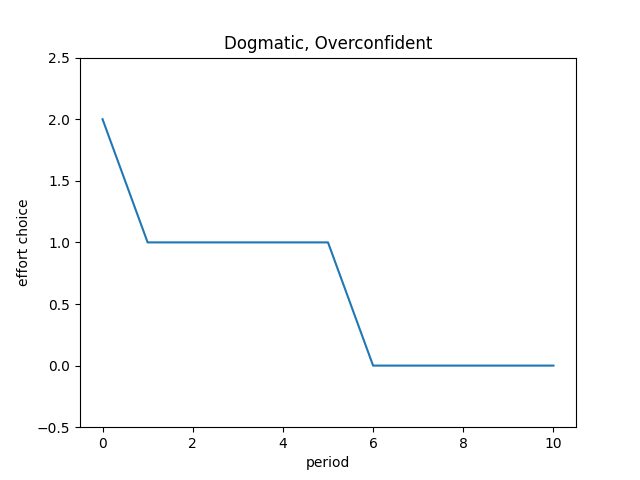
\includegraphics[scale=.5]{dogmatic_over_11.png}
        \caption{$\theta^*=\theta_M$, $\hat\theta=\theta_H$, $\omega^*=\omega_M$}
    \end{figure}
\end{frame}

\begin{frame}{The Switcher (paradigm shifts)}
    Same initial belief as the Dogmatic, but is willing to consider and alternative paradigm $\theta'$\\
    \bigskip
    Keeps track of the likelihoods of the two possible paradigms:\\
    \begin{itemize}
        \item $p(\cdot|h^t)$ for $\hat{\theta}$ and $\theta'$
    \end{itemize}
    \bigskip
    They swithch to whichever paradigm is morelikely to have generated the signals
    $$ \frac{p(\theta'|h^t)}{p(\hat{\theta}|h^t)}>\alpha\geq1$$
    
\end{frame}


\begin{frame}{The Switcher: Mechanism}
    

    \begin{enumerate}
        \item Chooses $e_H$ and is disappointed $\rightarrow$ adjust belief about $\omega$ downward\\
        \bigskip
        \item Eventually chooses $e_M$ and is disappointed as well $\rightarrow$ adjust belief about $\omega$\\
        \bigskip
        \item Eventually chooses $e_L$ and falls into a self-confirming equilibrium\\
        \bigskip
        \item At some point, the likelihood of $\theta_M$ becomes much larger than that of $\theta_H$ and the agent updates their belief
    \end{enumerate}
    
    
\end{frame}

\begin{frame}{Switcher Overconfident: Simulation}
    \begin{figure}
        \centering
        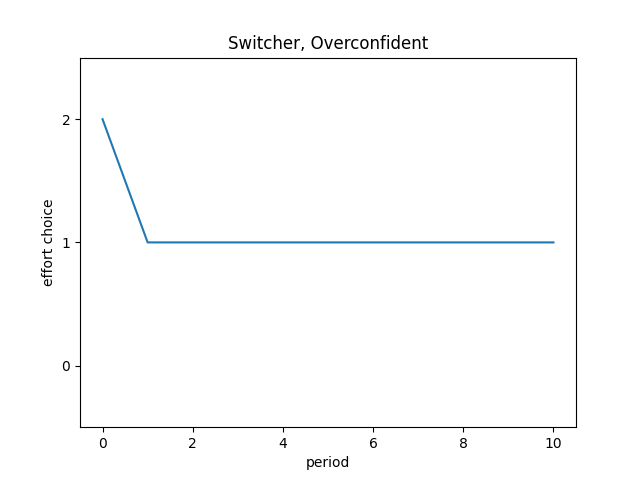
\includegraphics[scale=.5]{switcher_over_11.png}
        \caption{$\theta^*=\theta_M$, $\hat\theta=\theta_H$, $\omega^*=\omega_M$, $\alpha= 1.1$}
    \end{figure}
\end{frame}


\begin{frame}{Self-Attribution Bias / Optimal Expectations}
    Start with a diffused prior over $(\theta, \omega)$ but updates with a bias
    \begin{itemize}
        \item Success $\rightarrow$ overweight parametrizations with $\theta>\omega$\\
        \item Failure $\rightarrow$ underweight parametrizations with $\theta<\omega$\\
    \end{itemize}

    $$ p_{t+1}(\theta, \omega| s_t)=\frac{}{} $$
    

\end{frame}

\begin{frame}{Self-Attribution: Mechanism}
    \begin{enumerate}
        \item Chooses $e$ that maximizes utility according to priors
        \bigskip
        \item Belief on $\omega$ deteriorates a lot after bad news $\to$ big change in effort
        \item Belief on $\theta$ increases a lot after good news $\to$ small positive (or negative) change in effort \\
    \end{enumerate}
    
\end{frame}


\begin{frame}{Self-Attribution: Simulation}
        \begin{figure}
            \centering
            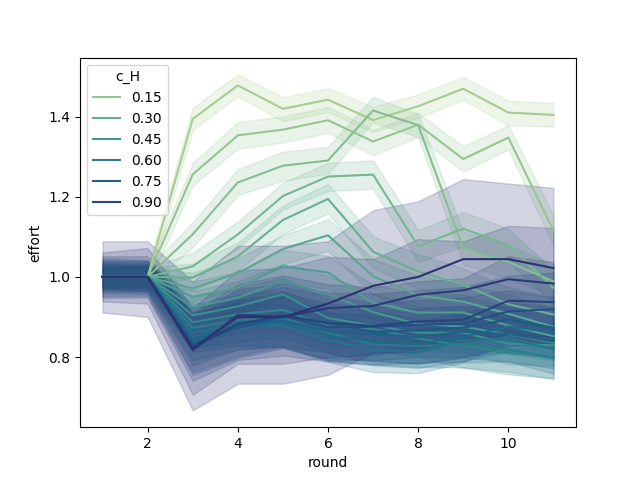
\includegraphics[scale=.5]{self-serving_11.png}
        
        \end{figure}
    \end{frame}

\begin{frame}{The Myopic Bayesian}
    
\end{frame}


    \begin{frame}{All Models}
    \label{Figure2}
        \begin{figure}
        \centering
        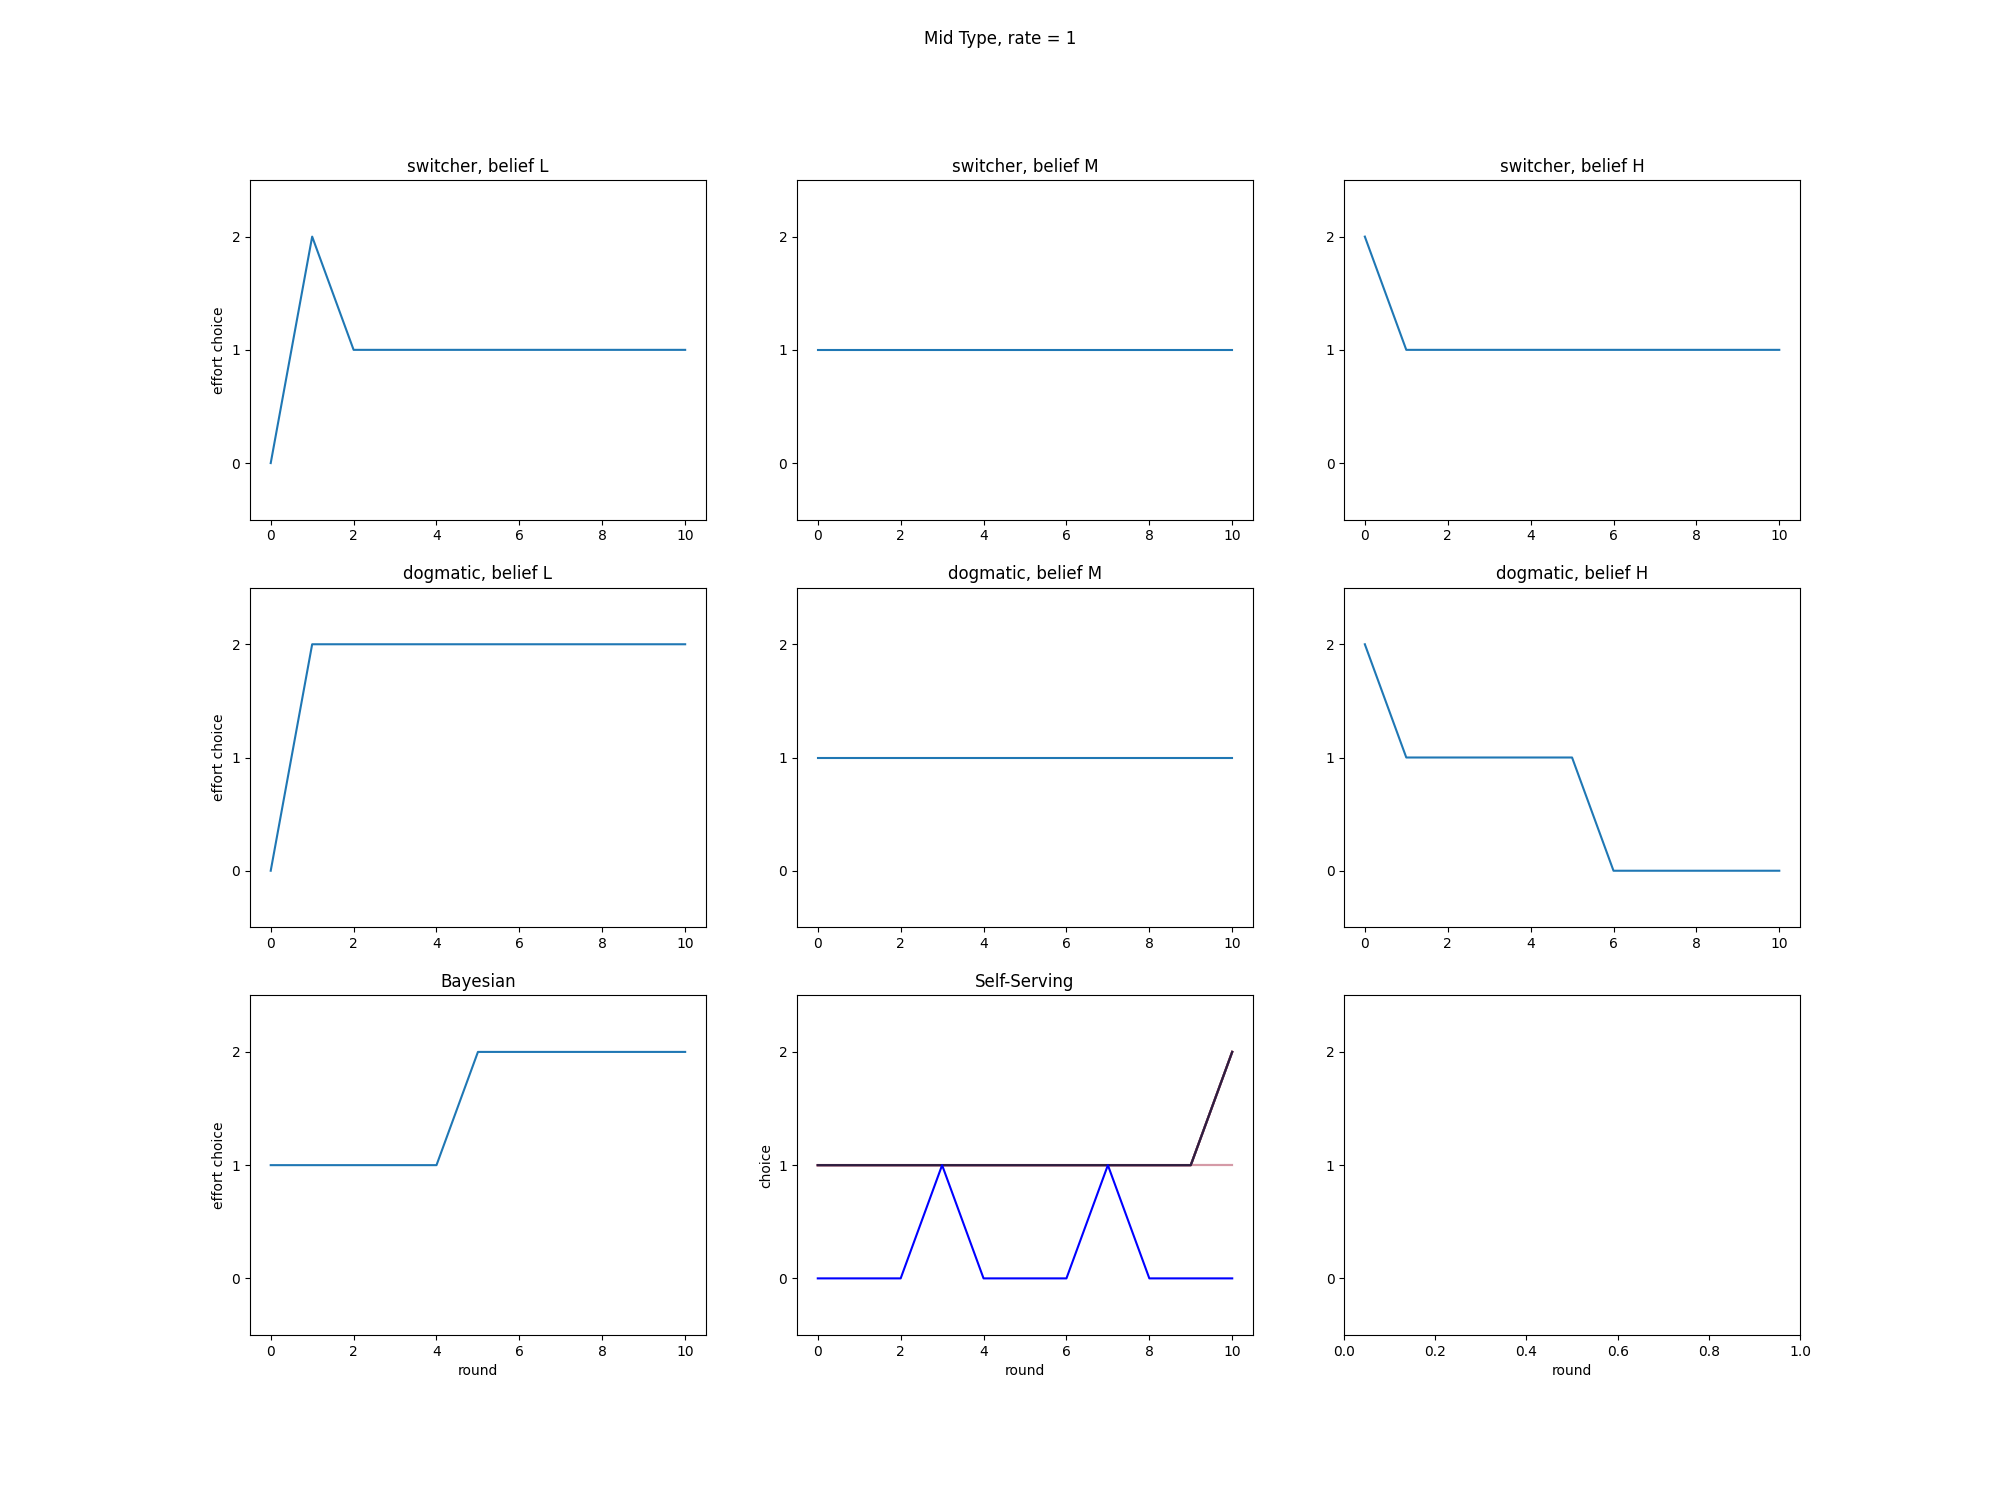
\includegraphics[scale=0.2]{all_11.png}
    \end{figure}     

\end{frame}

\section*{Experimental Design}

\begin{frame}{Set the Types}
    \bigskip
    \begin{itemize}
        \item Quiz: Answer as many questions as you can in 2 minutes\\
        \begin{itemize}
            \item Math, Verbal, Pop-Culture, Science, Us Geography, Sports and Video games\\
        \end{itemize}
        \bigskip

        \item How many questions do you think you answered correctly in each quiz?\\
        \begin{itemize}
            \item[o] 0 to 5
            \item 6 to 15 
            \item 16 or more
        \end{itemize}
        \item How sure are you about your choice?
        \begin{itemize}
            \item Random guess $\to 1/3$
            \item Another is equally likely $\to 1/2$
            \item Fairly certain $\to 3/4$
            \item Completely sure $\to 1$
        \end{itemize}
    \end{itemize}

\end{frame}


\begin{frame}{Choice and Update}
    Effort choice and feedback (One topic at a time)\\
    \bigskip
    \begin{itemize}
        \item Choose an effort
        \item Receive a sample of 10 signal realizations
    \end{itemize}
    \bigskip
    x 11 per topic

\end{frame}

\begin{frame}{Eliciting Beliefs?}
    \begin{itemize}
        \item $E[\omega]$ is revealed by their choice of effort\\
        \bigskip
        \item Eliciting beliefs for $\theta$ can incentivize learning in a way that is not consistent with the theory\\
        \bigskip
    \end{itemize}

    Allow them to see the success rate matrix for only one type. 
    \begin{itemize}
        \item Track the matrices they choose to see in each round
    \end{itemize}

\end{frame}

\begin{frame}{Stereotype condition}

    Observe the characteristics of a participant \\
    \begin{itemize}
        \item Gender, 
        \item US National or not \\
    \end{itemize}
    \bigskip
    Answer the same questions about slef and other\\

    \bigskip
    Belief updating and effort choice:\\
    \begin{itemize}
        \item  The DGP depends on the $\theta$ the other participant
    \end{itemize}
    \bigskip
    x 11 per topic

\end{frame}

\begin{frame}{Screen}
    \begin{figure}
        \centering
        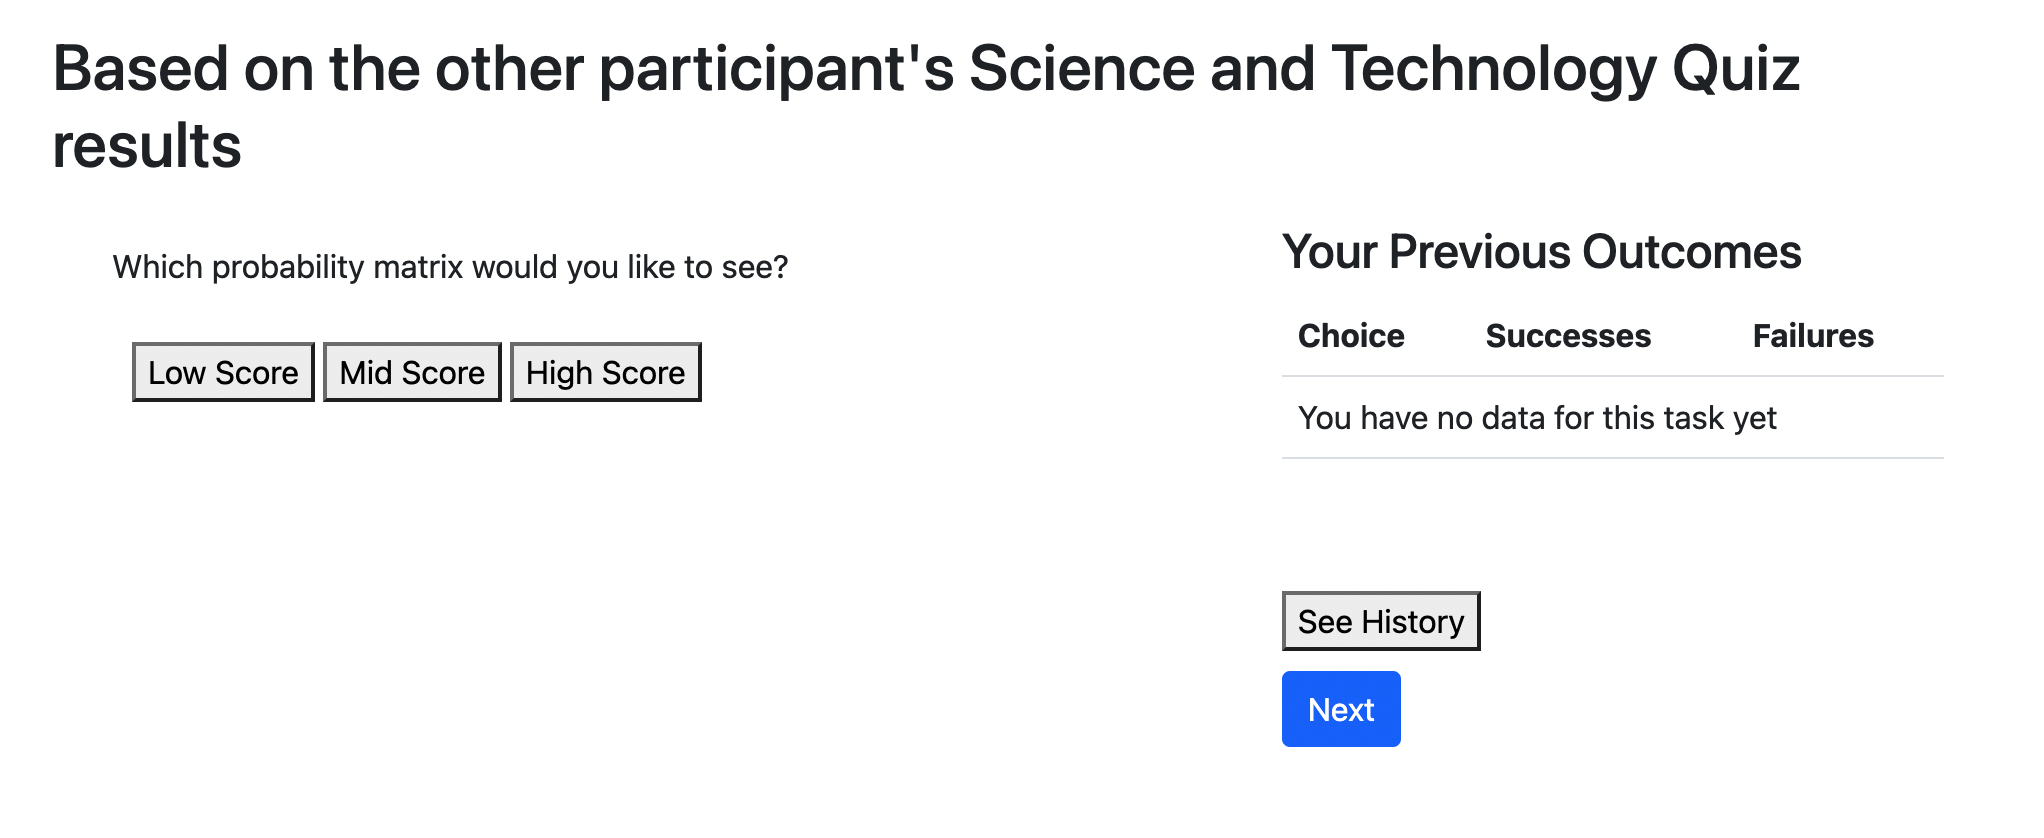
\includegraphics[scale=.4]{screen1.png}
    \end{figure}
\end{frame}

\begin{frame}{Screen}
    \begin{figure}
        \centering
        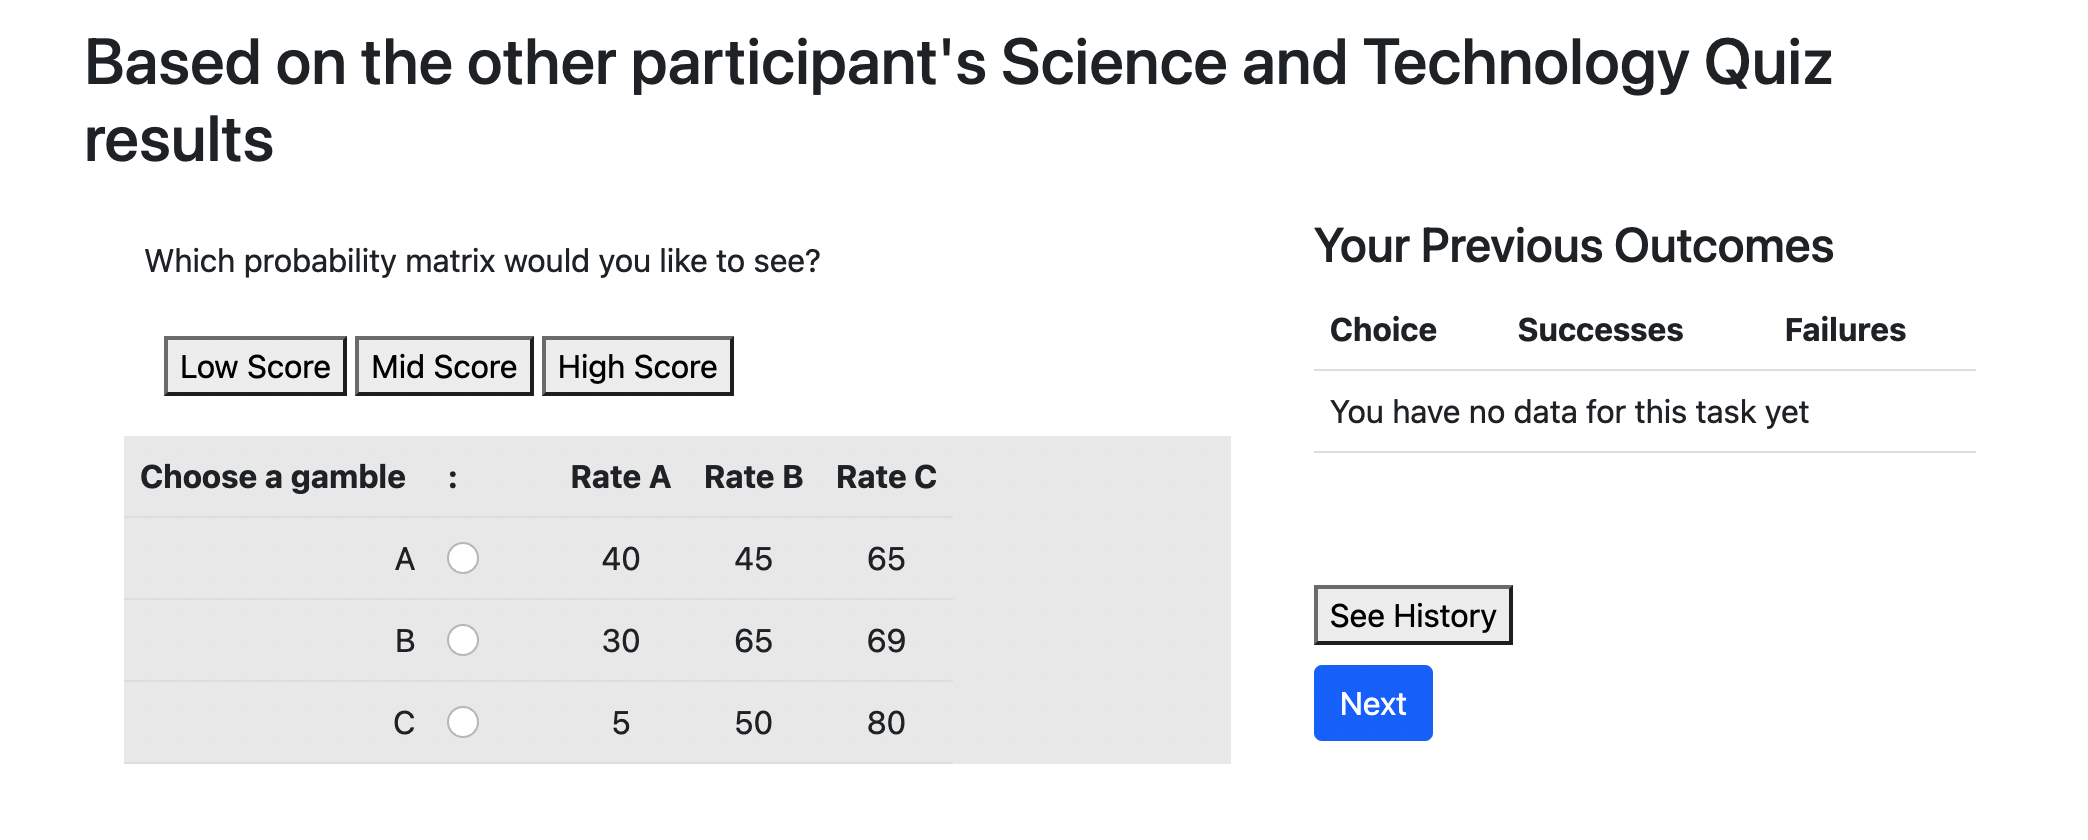
\includegraphics[scale=.4]{screen2.png}
    \end{figure}
\end{frame}

\section*{The Data}

\begin{frame}{The Data}
    Subject pool:\\
    \begin{itemize}
        \item Run at the CESS lab in person
        \item 45 subjects in Ego
        \item 33 subjects in Stereotype
    \end{itemize}
    \bigskip
    The Sessions:
    \begin{itemize}
        \item 8 sessions 
        \item 45 minutes on average
        \item Average payment: $\$23$
        \begin{itemize}
            \item $\$10$ show-up fee
            \item $\$ 0.20$ per correct answer
            \item $\$ 0.20$ per success
            \item Paid one topic at random
        \end{itemize}
    \end{itemize}
    
\end{frame}


\begin{frame}{Learning}
    

\end{frame}

\begin{frame}{Initial Misspecifications}
    

\end{frame}

\begin{frame}{The Stereotypes}


\end{frame}

\begin{frame}{Transitions}
    
\end{frame}

\section*{Parameter Estimation}

\begin{frame}{Identification of $\alpha$}
    

\end{frame}

\begin{frame}{Estimation of Self-Attribution Bias}
    
    
\end{frame}

\section*{Results}

\begin{frame}{Model Fit}
    
\end{frame}

\begin{frame}{Heterogeneity}
    
\end{frame}


\begin{frame}{The end}
    \large\textbf{Thank you!}
\end{frame}



\end{document}
